\documentclass[10pt]{beamer}

\usetheme[progressbar=frametitle]{metropolis}
\usepackage{appendixnumberbeamer}

\usepackage{booktabs}
\usepackage[scale=2]{ccicons}

\usepackage{pgfplots}
\usepgfplotslibrary{dateplot}

\usepackage{xspace}
\newcommand{\themename}{\textbf{\textsc{metropolis}}\xspace}

\usepackage{multimedia}
\usepackage{hyperref}
\usepackage{subcaption}

\graphicspath{ {figures/} }

\title{Tesselated Voxelization for Global Illumination using Voxel Cone Tracing}
%\subtitle{}
\date{June 2018}
\author{Sam Freed\\\\Committee Members:\\ Dr.\ Christian Eckhardt (chair), Dr.\ Maria Pantoja, Dr.\ Aaron Keen\\}
\institute{California Polytechnic State University, San Luis Obispo}
% \titlegraphic{\hfill\includegraphics[height=1.5cm]{logo.pdf}}

\AtBeginSection[]
{
	\begin{frame}
    	\frametitle{Outline}
        \tableofcontents[currentsection,hideothersubsections] % TODO show subsections/frames?
	\end{frame}
}

\begin{document}

\frame{\titlepage}

% Go over outlines of presentation. Mention the subsections briefly as appropriate.
\begin{frame}{Outline}
  \setbeamertemplate{section in toc}[sections numbered]
  \tableofcontents[hideallsubsections]
\end{frame}


\section{Introduction}

\begin{frame}{Introduction}
% who i am, thanks for coming, blah blah
\end{frame}

\begin{frame}{Teaser}
% video or screenshots, show good lighting + moving objects
\movie[autostart,showcontrols]{\textcolor{black}{\rule{\textwidth}{0.9\textheight}}}{test.webm}
\end{frame}

\begin{frame}{What did I just see?}
% real time gi of course!
\end{frame}

\subsection{Motivations}
\begin{frame}{Motivations}
  \begin{enumerate}
    \centering
    \item Real-time global illumination is difficult % lots of computation
    \item Limited reference material % open-source, cross-platform (-apple), no large engine, any documentation or explanation
    \pause
    \item I think it's cool % the real reason tbh
  \end{enumerate}
\end{frame}

\begin{frame}{Motivations}
  % Want to go from this...to _this_
  % \begin{columns}
  %   \begin{column}{0.5\textwidth}
      \begin{figure}
        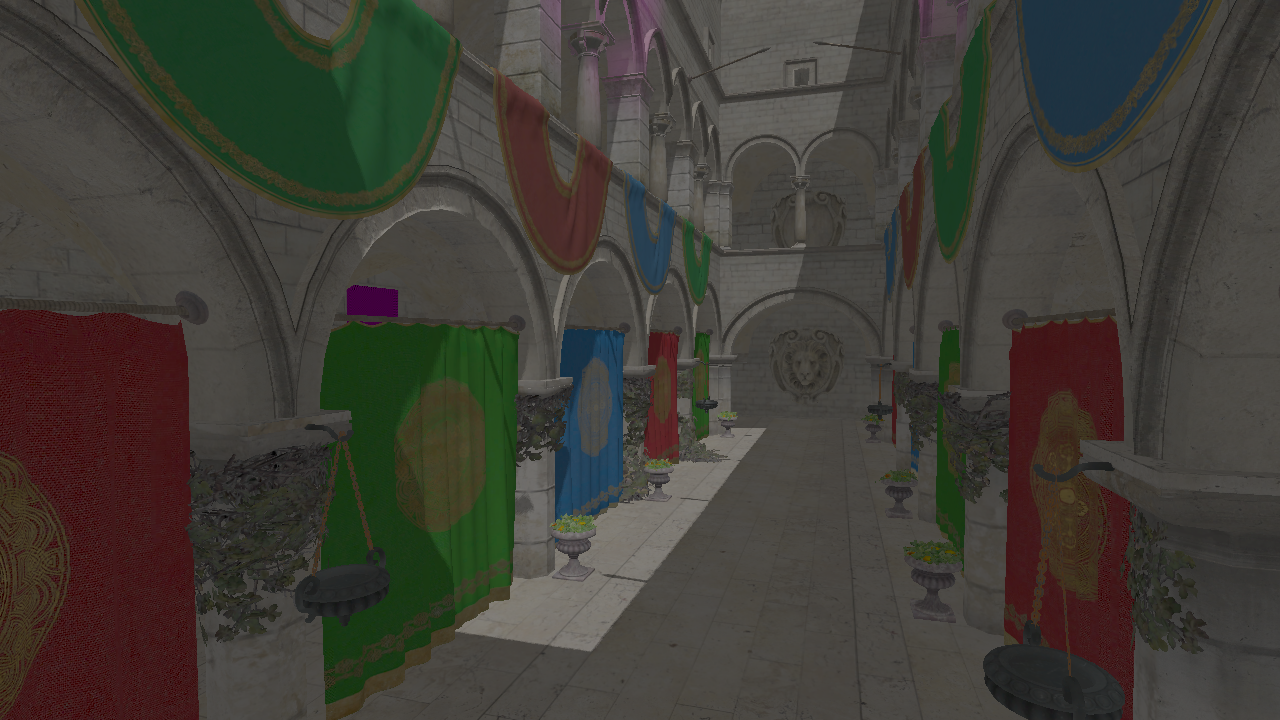
\includegraphics[width=\textwidth]{gi_off.png}
        :(
      \end{figure}
    \end{frame} \begin{frame}{Motivations}
  %   \end{column}
  %   \begin{column}{0.5\textwidth}
      \begin{figure}
        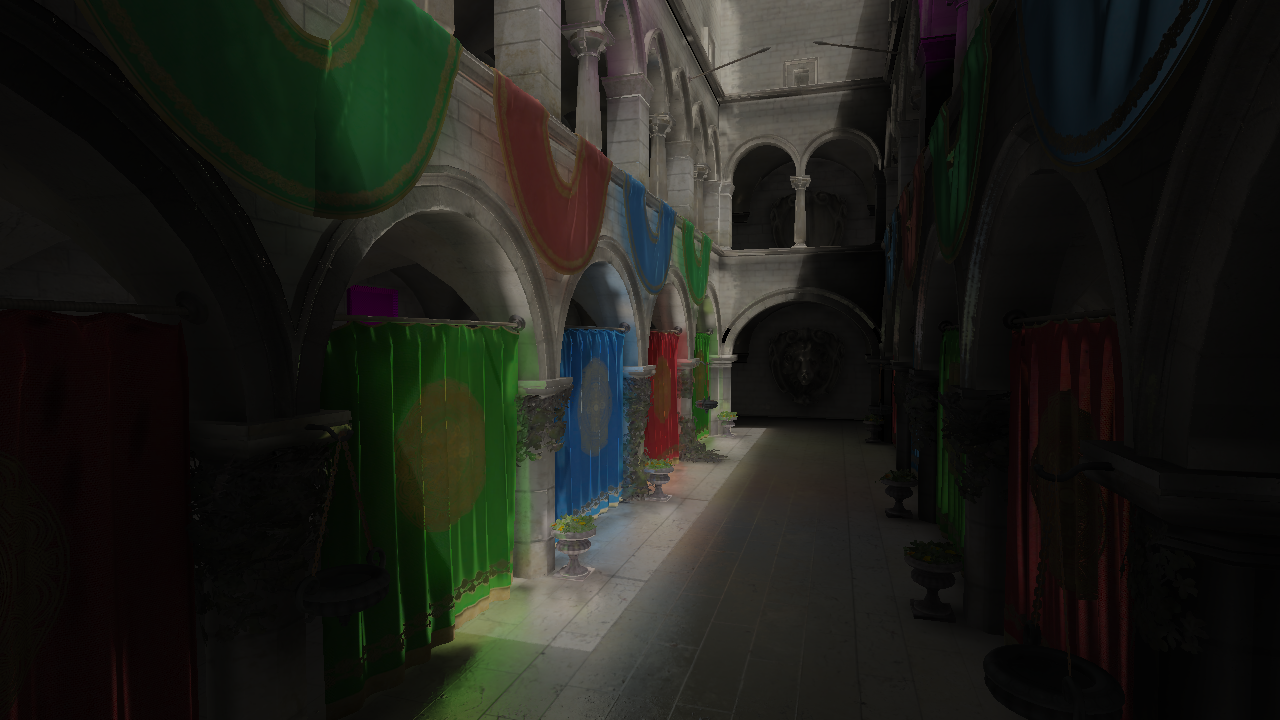
\includegraphics[width=\textwidth]{gi_on.png}
        :)
      \end{figure}
  %   \end{column}
  % \end{columns}
\end{frame}

\subsection{Contributions}
\begin{frame}{Contributions}
  \begin{itemize}
    \item Open-source, cross-platform implementation of global illumination using voxel cone tracing
    \item Detailed documentation on the algorithm and implementation % thesis and code comments "self documenting" :)
    \item Investigation into warped voxels and a comparison between raster and tesselation based voxelization
  \end{itemize}
\end{frame}


\section{Background}

\subsection{Computer Graphics}
\begin{frame}{Computer Graphics Primer}
  \begin{block}{Goal}
    Given a virtual description of a scene render an image.
  \end{block}

  \begin{block}{Big Issues}
    \begin{enumerate}
      \item How do we represent a scene? What information is required?  % geometry (triangles, voxels), materials (colors, properties), lights (type, position, color, direction), etc.
      \item How is a 3D scene represented as a 2D image?  % implies some transformation needed
      \item How do we `render'---how is the final pixel color computed? % lighting/shading model; this is the focus of this thesis
    \end{enumerate}
  \end{block}
  % rtr objects -> world space -> screen space
  % goal of computer graphics; graphics pipeline; transforms and other common stuff
\end{frame}

\begin{frame}{How do we represent a scene?}
  \setbeamercovered{transparent}
  \begin{columns}
    \begin{column}{0.5\textwidth}
      \begin{itemize}[<+->]
        \item Geometry: triangles, voxels % triangles inherently 2D->good for surfaces, not so much for volumetric data
        \item Materials: colors and other properties % like roughness, normal maps (kinda)
        \item Lights: positions, colors, etc.
      \end{itemize}
    \end{column}
    \begin{column}{0.5\textwidth}
      \only<1>{
        \begin{figure}
          \begin{subfigure}{\textwidth}
            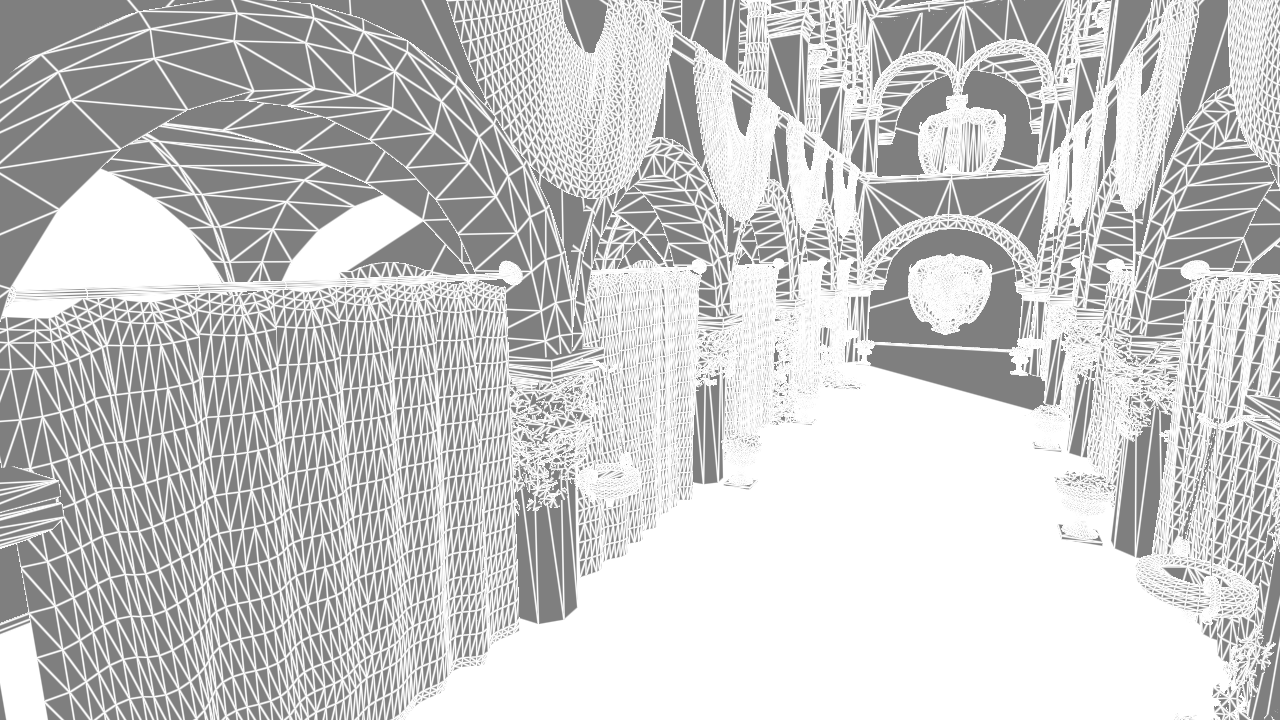
\includegraphics[width=\textwidth]{wireframe.png}
          \end{subfigure}
          \begin{subfigure}{\textwidth}
            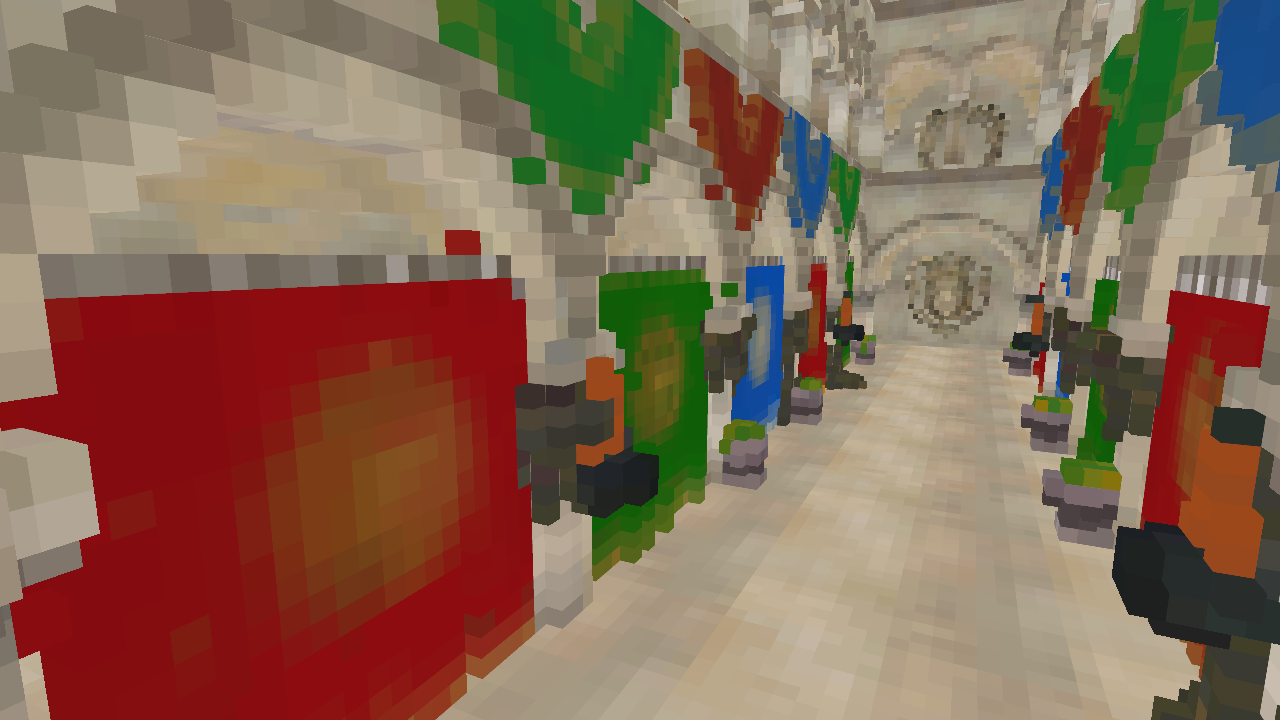
\includegraphics[width=\textwidth]{voxels.png}
          \end{subfigure}
        \end{figure}}

      \only<2>{
        \begin{figure}
          \begin{subfigure}{\textwidth}
            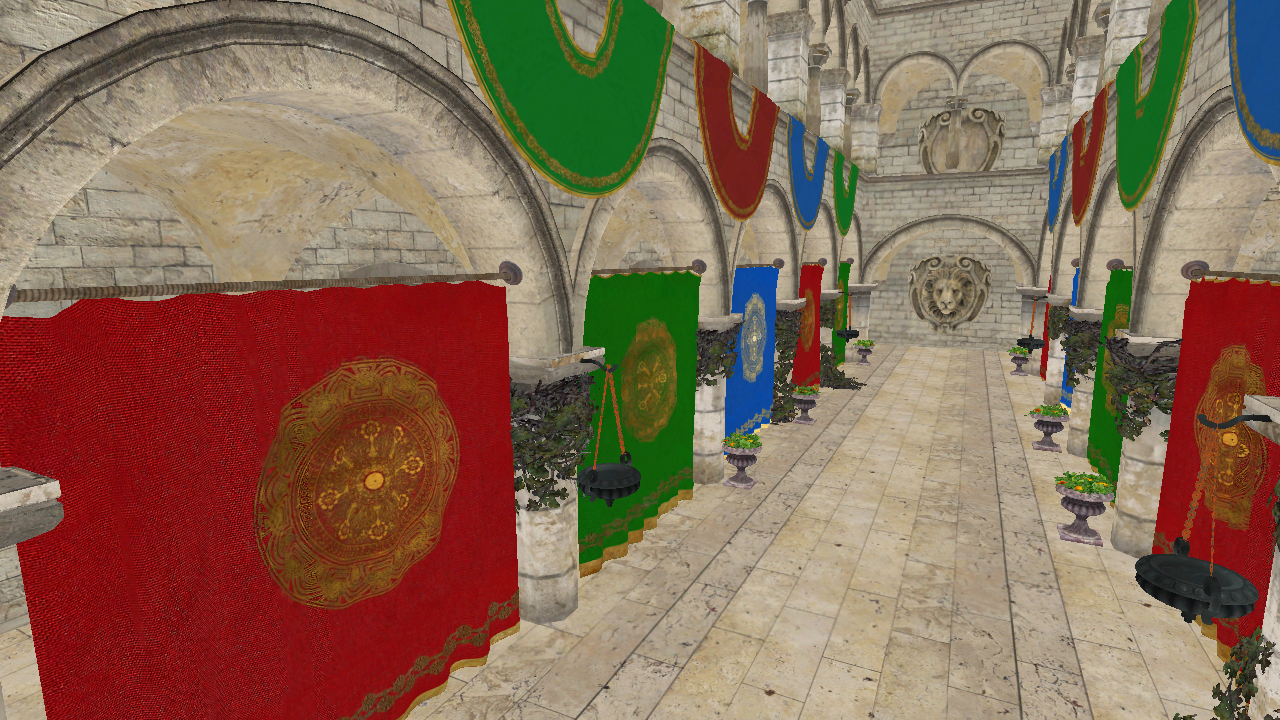
\includegraphics[width=\textwidth]{albedo.png}
          \end{subfigure}
          \begin{subfigure}{\textwidth}
            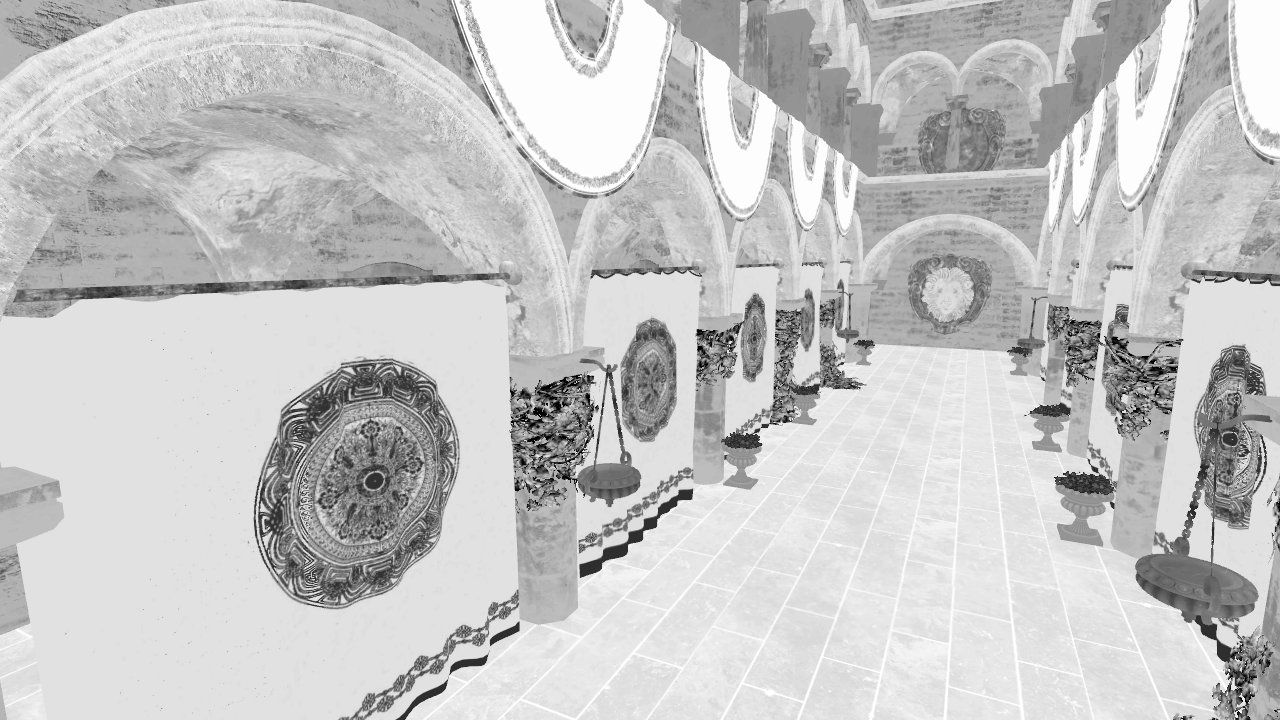
\includegraphics[width=\textwidth]{roughness.png}
          \end{subfigure}
        \end{figure}}

      \only<3>{
        \begin{figure}
          \begin{subfigure}{\textwidth}
            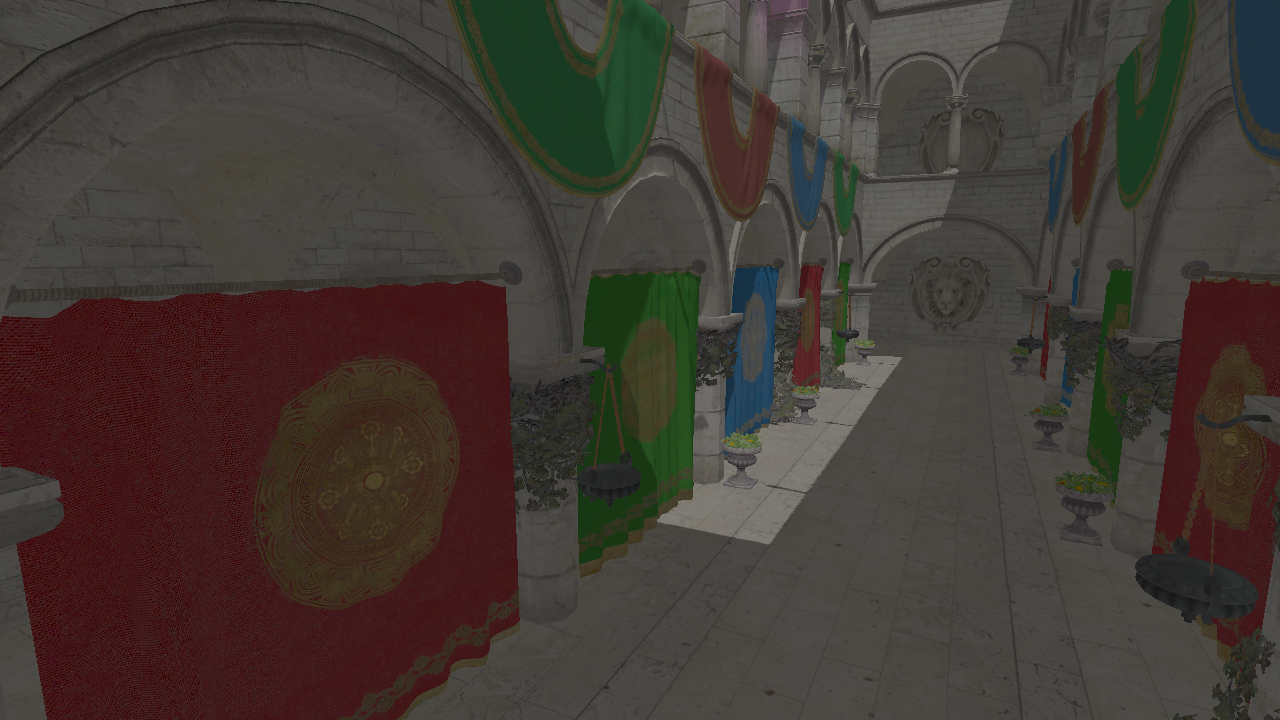
\includegraphics[width=\textwidth]{nogi.png}
          \end{subfigure}
          \begin{subfigure}{\textwidth}
            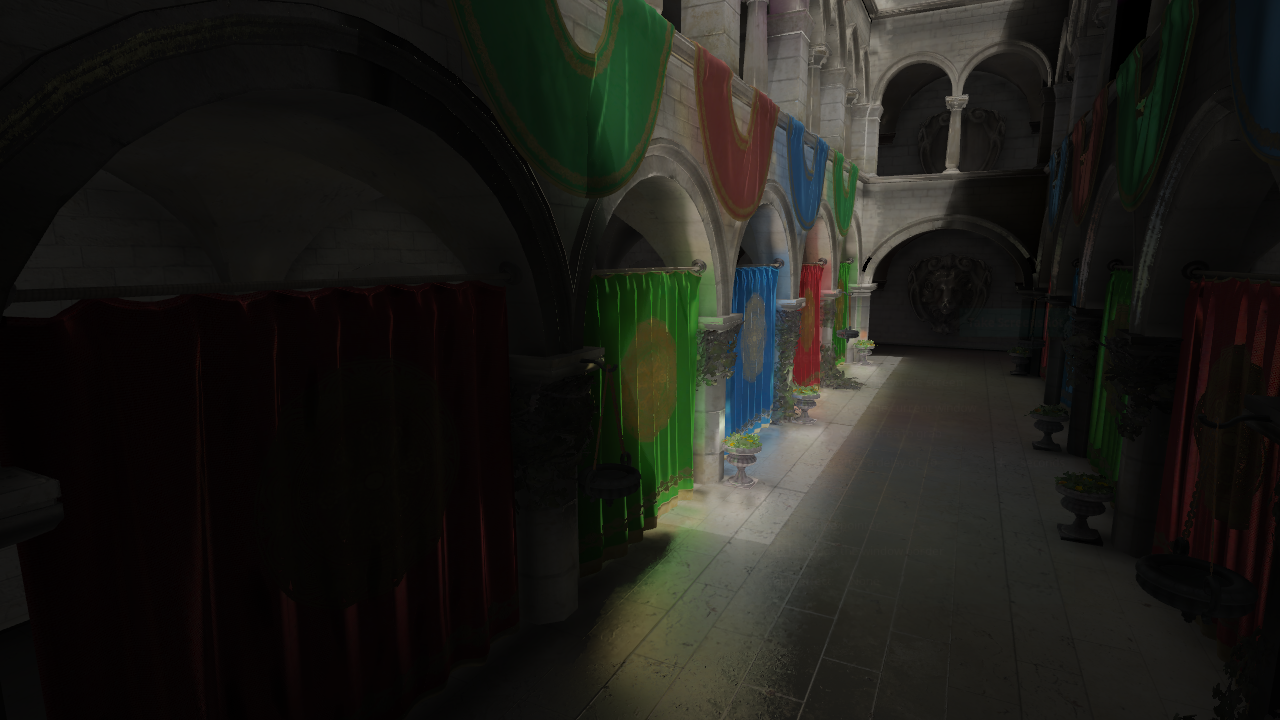
\includegraphics[width=\textwidth]{gi.png}
          \end{subfigure}
        \end{figure}}
    \end{column}
  \end{columns}
\end{frame}

{\setbeamertemplate{frame footer}{image from Real-Time Rendering} % TODO cite
\begin{frame}{How is a 3D scene represented as a 2D image?}
  Math!

  All coordinates are transformed multiple times before ending up at their appropriate place on the screen.

  \begin{figure}
    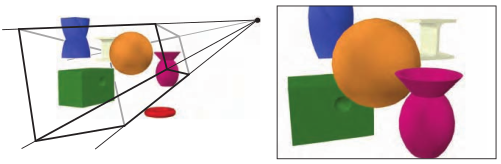
\includegraphics[width=\textwidth]{rtr_fig2_1.png}
  \end{figure}

\end{frame}}


\begin{frame}{How is a 3D scene represented as a 2D image?}
  % picture of coordinate systems and give brief explanation, since explain more along with the graphics pipeline
  % showing this so everyone is comfortable when explaining algorithms
  % ...and this is accomplished with <flick> THE GRAPHICS PIPELIIIIIIINE

  \begin{figure}
    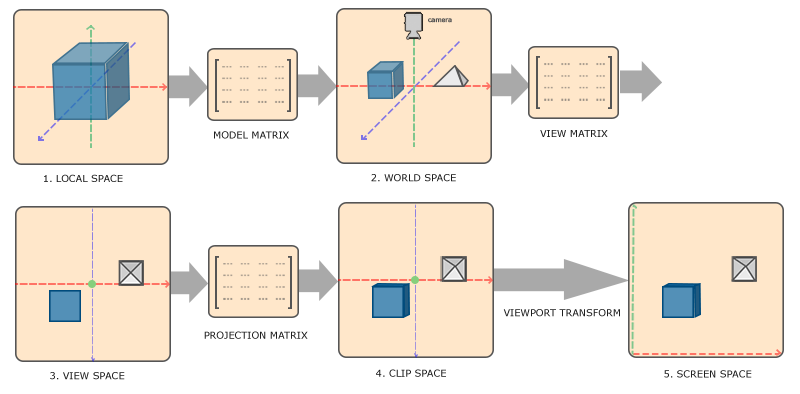
\includegraphics[width=\textwidth]{learnopengl_coordinate_systems.png}
  \end{figure}

  \begin{description}[<+| only@+>]
    \item[Local/Object Space] coordinate system relative to a single object
    \item[World Space] a global coordinate system for the virtual world
    \item[View Space] coordinates are with respect to the camera
    \item[Clip Space/NDC] defines a frustum in which objects will be rasterized % those outside the frustum are clipped
    \item[Screen Space] coordinates are the pixel position and a depth value
  \end{description}

  % Also other spaces, like texture space [0, 1], image space (integral coordinates),

\end{frame}

\begin{frame}{How is a 3D scene represented as a 2D image?}
  \begin{center}
    \huge\textbf{The Graphics Pipeline}
  \end{center}
  % picture of pipeline
  % This is the standard sequence of events that render the final image from our scene
  % We'll go over the entire pipeline for sake of completess

  \begin{figure}
    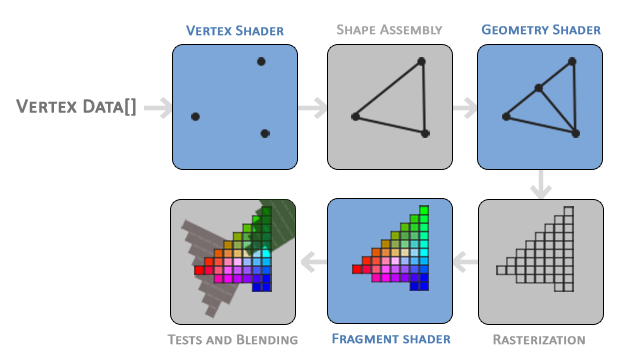
\includegraphics[width=\textwidth]{learnopengl_graphicspipeline.png}
  \end{figure}
\end{frame}

\begin{frame}{Graphics Pipeline---Input}
  A series of vertices, containing attributes like position, normal, texture coordinates, etc.
\end{frame}

\begin{frame}{Graphics Pipeline---Vertex Shading}

\end{frame}

\begin{frame}{Graphics Pipeline---Shape Assembly}

\end{frame}

\begin{frame}{Graphics Pipeline---Geometry Shading}

\end{frame}

\begin{frame}{Graphics Pipeline---Rasterization}

\end{frame}

\begin{frame}{Graphics Pipeline---Fragment Shading}

\end{frame}

\begin{frame}{Graphics Pipeline---Testing and Blending}

\end{frame}

\begin{frame}{Compute Shader}
  % just want to introduce the concept since I'll mention them in implementation
\end{frame}

\begin{frame}{Tesselation}
  % briefly go over triangle tesselation and where it fits in the pipeline. will probably talk about it more in implementation
\end{frame}

\begin{frame}{Spatial Data Structures}
  % quickly go through one slide each (with picture)
\end{frame}

\begin{frame}{How do we `render'?}
  % We need a shading model: a way to compute a color from the geometry, lights, and materials we have in the scene for a particular point
  % Makes sense to model this based on the real-world sooo
  % See the next section!
\end{frame}

\subsection{Lighting}
\begin{frame}{Radiance and the Rendering Equation}
  % Semi-detailed, need to have audience at least have some idea what's going on
  % Note how this is computationally intensive -> need to resort to approximations
\end{frame}

\begin{frame}{Direct Lighting}
  % use as example of how lighting works, some intuition on rendering equation
  % should help to understand indirect lighting
\end{frame}

\begin{frame}{Indirect Lighting}
  % what is is, other approaches, general approaches?
\end{frame}

% ask for any questions or clarification here? (after related work too maybe?)

\section{Related Work}

\subsection{VPLs and RSMs}
\begin{frame}{VPLs and RSMs}
  % Just want to introduce the concept of VPLs and RSMs are simple way of doing that
  \begin{description}
    \item[Virtual Point Lights:] Treat arbitrary objects or locations as light sources.
    \item[Reflective Shadow Maps:] Treat each pixel of a shadowmap as a VPL. % when rendering project point into shadowmap and gather lighting contributions from VPLs; problem is poor occlusion information and only low frequency lighting
  \end{description}
\end{frame}

\subsection{Light Propogation Volumes}
\begin{frame}{Light Propogation Volumes}
  % low frequency but fairly stable, no occlusion (limited info from reusing), cascaded
\end{frame}

\subsection{Voxel Cone Tracing}
\begin{frame}{Voxel Cone Tracing}
  % complete occlusion info, sparse voxel octree, specular reflections
\end{frame}


\section{Implementation}

\begin{frame}{Overview of Renderer}
  % flowchart or something showing each render pass
\end{frame}

\subsection{Voxelization}
\begin{frame}{Voxelization with Rasterizer}
  % main idea: rasterized fragments correspond to voxel
  % setup: need projection matrices
  % geometry shader: choose dominant axis and project
  % fragment shader:
\end{frame}

\begin{frame}{Voxelization with Tesselator}
\end{frame}

\subsection{Radiance Injection and Filtering}
\begin{frame}{Radiance Injection}
  \begin{block}{Goal}
    Create virtual point lights for all geometry hit by the light.

    These lights approximate a single-bounce of indirect lighting.
  \end{block}

  Another voxel texture stores the locations of these VPLs.
\end{frame}

\begin{frame}{Radiance Injection---Shadow Mapping}
  To determine where the virtual point lights should be, we use a \textbf{shadowmap}.

  Render the scene from the \textit{light}'s point of view.

  Only interested in depth values % important for us: along with the light matrix we can reconstruct world positions
  % picture
  \footnote{An RSM could be made by also saving surface color and normal.}

  % implementation? ortho matrix, projection
\end{frame}

\begin{frame}{Radiance Injection---Injecting VPLs}
  For each pixel in the shadowmap, find it's voxel index and insert the corresponding color into the radiance texture.

  Using the light matrix and stored depth value, we compute the point's world space position.
\end{frame}

\begin{frame}{Radiance Filtering}
  Radiance texture contains multiple \textbf{levels} (mipmaps). Each level is half the size of the previous. A compute shader performs a 2x2x2 box filter for each level to determine the filtered value.

  % show 2D box filter
  % show the four images
\end{frame}

\subsection{Final Shading}
\begin{frame}{Depth Prepass}
  An optimization to minimize the number of shaded fragments.

  Prefill the depth buffer so lighting (including the relatively expensive voxel cone tracing) will only be performed on the visible fragments of the scene. % remind of depth test
\end{frame}

\begin{frame}{Final Shading}
  % outline (direct + diffuse indirect + specular indirect)
  % inputs are lights, material, and fragment (with position, normal, texture coordinates)
\end{frame}

\begin{frame}{Direct Lighting}
  % cook torrance too?
  % don't forget shadows
\end{frame}

\begin{frame}{Indirect Lighting}
% explain voxel cone tracing
% the idea (raymarching + mipmaps), choosing cone angles + dirs, diffuse indirect, specular indirect, cone tracing itself
\end{frame}

\subsection{Voxel Warping}
\begin{frame}{Voxel Warping}
\end{frame}


\section{Results}

\begin{frame}{Screenshots}
\end{frame}

\begin{frame}{Performance \& Memory Usage}
\end{frame}

\begin{frame}{Validation}
  % explain difficulties in comparing to others but still give numbers or something
\end{frame}


\section{Conclusion}

{\setbeamertemplate{frame footer}{*Find the source here: \url{github.com/sfreed141/vct}}
\begin{frame}{Conclusion}
\end{frame}}

\begin{frame}{Future Work}
\end{frame}

\begin{frame}{}
  \begin{center}
    \LARGE Thank you!
  \end{center}
\end{frame}

\begin{frame}{}
  \begin{center}
    \LARGE Questions?
  \end{center}
\end{frame}

% TODO bibliography slides?

\section{Elements}

\begin{frame}[fragile]{Typography}
      \begin{verbatim}The theme provides sensible defaults to
\emph{emphasize} text, \alert{accent} parts
or show \textbf{bold} results.\end{verbatim}

  \begin{center}becomes\end{center}

  The theme provides sensible defaults to \emph{emphasize} text,
  \alert{accent} parts or show \textbf{bold} results.
\end{frame}

\begin{frame}{Font feature test}
  \begin{itemize}
    \item Regular
    \item \textit{Italic}
    \item \textsc{SmallCaps}
    \item \textbf{Bold}
    \item \textbf{\textit{Bold Italic}}
    \item \textbf{\textsc{Bold SmallCaps}}
    \item \texttt{Monospace}
    \item \texttt{\textit{Monospace Italic}}
    \item \texttt{\textbf{Monospace Bold}}
    \item \texttt{\textbf{\textit{Monospace Bold Italic}}}
  \end{itemize}
\end{frame}

\begin{frame}{Lists}
  \begin{columns}[T,onlytextwidth]
    \column{0.33\textwidth}
      Items
      \begin{itemize}
        \item Milk \item Eggs \item Potatos
      \end{itemize}

    \column{0.33\textwidth}
      Enumerations
      \begin{enumerate}
        \item First, \item Second and \item Last.
      \end{enumerate}

    \column{0.33\textwidth}
      Descriptions
      \begin{description}
        \item[PowerPoint] Meeh. \item[Beamer] Yeeeha.
      \end{description}
  \end{columns}
\end{frame}

\begin{frame}{Figures}
  \begin{figure}
    \newcounter{density}
    \setcounter{density}{20}
    \begin{tikzpicture}
      \def\couleur{alerted text.fg}
      \path[coordinate] (0,0)  coordinate(A)
                  ++( 90:5cm) coordinate(B)
                  ++(0:5cm) coordinate(C)
                  ++(-90:5cm) coordinate(D);
      \draw[fill=\couleur!\thedensity] (A) -- (B) -- (C) --(D) -- cycle;
      \foreach \x in {1,...,40}{%
          \pgfmathsetcounter{density}{\thedensity+20}
          \setcounter{density}{\thedensity}
          \path[coordinate] coordinate(X) at (A){};
          \path[coordinate] (A) -- (B) coordinate[pos=.10](A)
                              -- (C) coordinate[pos=.10](B)
                              -- (D) coordinate[pos=.10](C)
                              -- (X) coordinate[pos=.10](D);
          \draw[fill=\couleur!\thedensity] (A)--(B)--(C)-- (D) -- cycle;
      }
    \end{tikzpicture}
    \caption{Rotated square from
    \href{http://www.texample.net/tikz/examples/rotated-polygons/}{texample.net}.}
  \end{figure}
\end{frame}

\begin{frame}{Tables}
  \begin{table}
    \caption{Largest cities in the world (source: Wikipedia)}
    \begin{tabular}{lr}
      \toprule
      City & Population\\
      \midrule
      Mexico City & 20,116,842\\
      Shanghai & 19,210,000\\
      Peking & 15,796,450\\
      Istanbul & 14,160,467\\
      \bottomrule
    \end{tabular}
  \end{table}
\end{frame}

\begin{frame}{Blocks}
  Three different block environments are pre-defined and may be styled with an
  optional background color.

  \begin{columns}[T,onlytextwidth]
    \column{0.5\textwidth}
      \begin{block}{Default}
        Block content.
      \end{block}

      \begin{alertblock}{Alert}
        Block content.
      \end{alertblock}

      \begin{exampleblock}{Example}
        Block content.
      \end{exampleblock}

    \column{0.5\textwidth}

      \metroset{block=fill}

      \begin{block}{Default}
        Block content.
      \end{block}

      \begin{alertblock}{Alert}
        Block content.
      \end{alertblock}

      \begin{exampleblock}{Example}
        Block content.
      \end{exampleblock}

  \end{columns}
\end{frame}

\begin{frame}{Math}
  \begin{equation*}
    e = \lim_{n\to \infty} \left(1 + \frac{1}{n}\right)^n
  \end{equation*}
\end{frame}
\begin{frame}{Line plots}
  \begin{figure}
    \begin{tikzpicture}
      \begin{axis}[
        mlineplot,
        width=0.9\textwidth,
        height=6cm,
      ]

        \addplot {sin(deg(x))};
        \addplot+[samples=100] {sin(deg(2*x))};

      \end{axis}
    \end{tikzpicture}
  \end{figure}
\end{frame}

\begin{frame}{Bar charts}
  \begin{figure}
    \begin{tikzpicture}
      \begin{axis}[
        mbarplot,
        xlabel={Foo},
        ylabel={Bar},
        width=0.9\textwidth,
        height=6cm,
      ]

      \addplot plot coordinates {(1, 20) (2, 25) (3, 22.4) (4, 12.4)};
      \addplot plot coordinates {(1, 18) (2, 24) (3, 23.5) (4, 13.2)};
      \addplot plot coordinates {(1, 10) (2, 19) (3, 25) (4, 15.2)};

      \legend{lorem, ipsum, dolor}

      \end{axis}
    \end{tikzpicture}
  \end{figure}
\end{frame}

\begin{frame}{Quotes}
  \begin{quote}
    Veni, Vidi, Vici
  \end{quote}
\end{frame}

\begin{frame}{References}
  Some references to showcase [allowframebreaks] \cite{knuth92,ConcreteMath,Simpson,Er01,greenwade93}
\end{frame}

\appendix

\begin{frame}[fragile]{Backup slides}
  Sometimes, it is useful to add slides at the end of your presentation to
  refer to during audience questions.

  The best way to do this is to include the \verb|appendixnumberbeamer|
  package in your preamble and call \verb|\appendix| before your backup slides.

  \themename will automatically turn off slide numbering and progress bars for
  slides in the appendix.
\end{frame}

\begin{frame}[allowframebreaks]{References}

  \bibliography{demo}
  \bibliographystyle{abbrv}

\end{frame}

\end{document}
